\documentclass[compress]{beamer}
\usepackage{ifthen,verbatim}

\newcommand{\isnote}{}
\xdefinecolor{lightyellow}{rgb}{1.,1.,0.25}
\xdefinecolor{darkblue}{rgb}{0.1,0.1,0.7}
\xdefinecolor{darkgreen}{rgb}{0.1,0.6,0.1}

%% Uncomment this to get annotations
%% \def\notes{\addtocounter{page}{-1}
%%            \renewcommand{\isnote}{*}
%% 	   \beamertemplateshadingbackground{lightyellow}{white}
%%            \begin{frame}
%%            \frametitle{Notes for the previous page (page \insertpagenumber)}
%%            \itemize}
%% \def\endnotes{\enditemize
%% 	      \end{frame}
%%               \beamertemplateshadingbackground{white}{white}
%%               \renewcommand{\isnote}{}}

%% Uncomment this to not get annotations
\def\notes{\comment}
\def\endnotes{\endcomment}

\setbeamertemplate{navigation symbols}{}
\setbeamertemplate{headline}{\mbox{ } \hfill
\begin{minipage}{5.5 cm}
\vspace{-0.75 cm} \small
\end{minipage} \hfill
\begin{minipage}{4.5 cm}
\vspace{-0.75 cm} \small
\begin{flushright}
\ifthenelse{\equal{\insertpagenumber}{1}}{}{Jim Pivarski \hspace{0.2 cm} \insertpagenumber\isnote/\pageref{numpages}}
\end{flushright}
\end{minipage}\mbox{\hspace{0.2 cm}}\includegraphics[height=1 cm]{../cmslogo} \hspace{0.1 cm} \includegraphics[height=1 cm]{../tamulogo} \hspace{0.01 cm} \vspace{-1.05 cm}}

\begin{document}
\begin{frame}
\vfill
\begin{center}
\textcolor{darkblue}{\Large Status of Muon Endcap Alignment}

\vfill
\begin{columns}
\column{0.3\linewidth}
\begin{center}
\large
\textcolor{darkblue}{Jim Pivarski}

\vspace{0.2 cm}
Alexei Safonov
\end{center}

\column{0.3\linewidth}
\begin{center}
\large
K\'aroly Banicz
\end{center}
\end{columns}

\begin{columns}
\column{0.3\linewidth}
\begin{center}
\scriptsize
{\it Texas A\&M University}
\end{center}
\column{0.3\linewidth}
\begin{center}
\scriptsize
{\it US-CMS}
\end{center}
\end{columns}

\vfill
 8 August, 2008

\end{center}
\end{frame}

%% \begin{notes}
%% \item This is the annotated version of my talk.
%% \item If you want the version that I am presenting, download the one
%% labeled ``slides'' on Indico (or just ignore these yellow pages).
%% \item The annotated version is provided for extra detail and a written
%% record of comments that I intend to make orally.
%% \item Yellow notes refer to the content on the {\it previous} page.
%% \item All other slides are identical for the two versions.
%% \end{notes}

\begin{frame}
\frametitle{Outline}
\vspace{-1.3 cm}
\begin{itemize}\setlength{\itemsep}{0.75 cm}
\item Update on CSC-Overlaps procedure 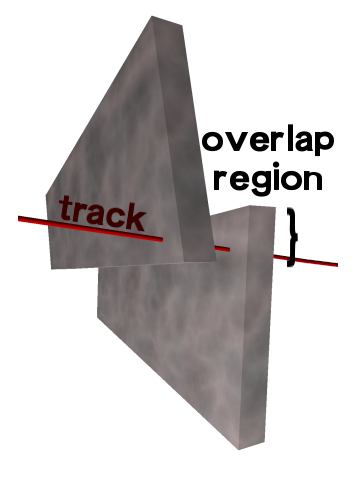
\includegraphics[height=2.5 cm]{overlaps.png}
\item Alignment of endcap disks in CRUZETs 1\&2
\item Discovery and correction of ideal-geometry mistake
\item New AlCaReco streams for CRUZET-4/CRAFT
\end{itemize}
%% \hspace{-0.83 cm} \textcolor{darkblue}{\Large Outline2}
\end{frame}

\begin{frame}
\frametitle{Update on CSC-Overlaps}
\small

\vspace{0.3 cm}
\hspace{-0.5 cm} ME+2/2 in CRUZET-1: \textcolor{red}{red arrows} and \textcolor{darkgreen}{green points} are \mbox{both the $x$ alignment\hspace{-1 cm}}

\vspace{-0.3 cm}
\begin{center}
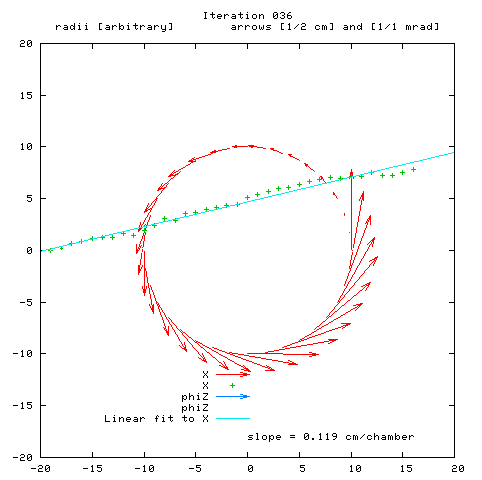
\includegraphics[height=5.5 cm]{frame36.png}
\end{center}

\vspace{-0.3 cm}
\begin{itemize}
\item \small converges: residuals become centered and alignment slows to a stop
\item \small ring overcloses by 4~cm due to 1.2~mm systematic error per chamber
\item \small same pattern in CRUZET-2, fit other direction, fit both $x$ and $\phi_z$\ldots
\end{itemize}
\end{frame}

\begin{frame}
\frametitle{Sources of systematics}
\small
All information is local: very little averaging over instrumental effects
\begin{enumerate}
\item Last strip is unique: no charge-sharing without a neighbor
\item Local $x$ is not a good measurement near the edges
\end{enumerate}

\vfill
\begin{columns}
\column{0.28\linewidth}

%% \vspace{0.2 cm}
\mbox{ } \hfill 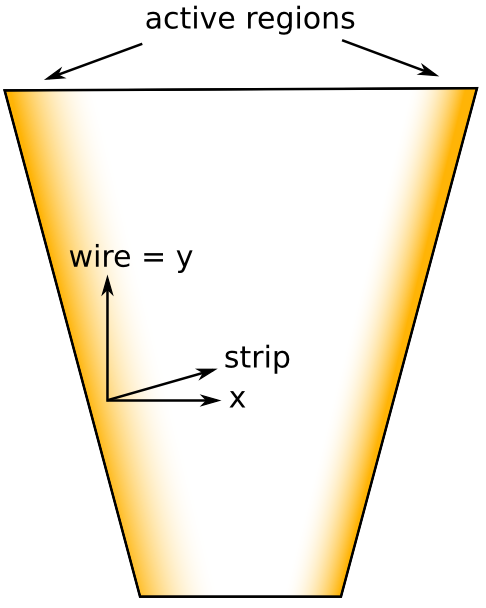
\includegraphics[width=\linewidth]{directions.png} \hfill \mbox{ }

%% \vspace{0.5 cm}
%% 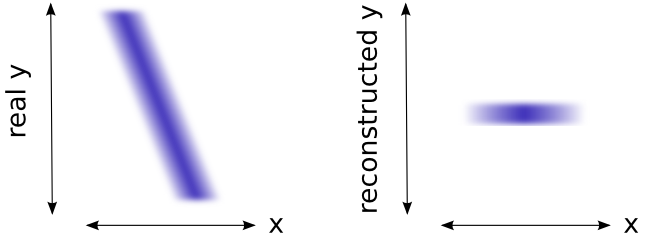
\includegraphics[width=\linewidth]{ignorance_of_y.png}

\column{0.7\linewidth}
\textcolor{darkblue}{\#2} in more detail:
\begin{itemize}
\item Local $x$ has a large component from wire measurement near the edges
\item Wires are ganged into 5~cm tall groups, position is taken to be the center of the group
\item Hit position has a discrete component, fit from neighboring chamber has a discrete component, the two are offset (and angled)
\item Can bias $x$ residuals by $\mathcal{O}($mm$)$ with the observed pattern
\end{itemize}
\end{columns}

\vfill
Modifying procedure to use pure strip measurements, rather than local $x$
\end{frame}

\begin{frame}
\frametitle{Alignment of endcap disks}

\begin{itemize}
\item Completed for CRUZETs 1\&2, awaiting re-reco of CRUZET-3
\item Modification of MuonHIP procedure to use StandAloneMuons
\end{itemize}

\begin{center}
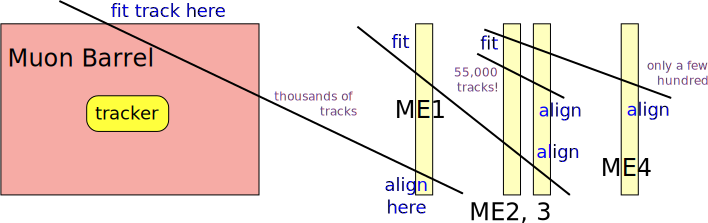
\includegraphics[width=0.9\linewidth]{fit_here_align_there}
\end{center}

\begin{itemize}
\item Muon barrel is the reference (aligned by Pablo)
\item Internal cross-checks by comparing direct MB$\to$ME2

against MB$\to$ME1 $+$ ME1$\to$ME2 (etc.)

\item Whole disks are the alignables, ``misalignments'' are huge because the detector is open
\end{itemize}
\end{frame}

\begin{frame}
\frametitle{Deconstructed alignment}

\begin{itemize}
\item Tools designed for many alignables and small misalignments
\item We have 4 alignables, misaligned by {\it meters}
\item Start with a pedestrian approach: hit-by-hit ntuple
\end{itemize}

\begin{columns}
\column{0.6\linewidth}
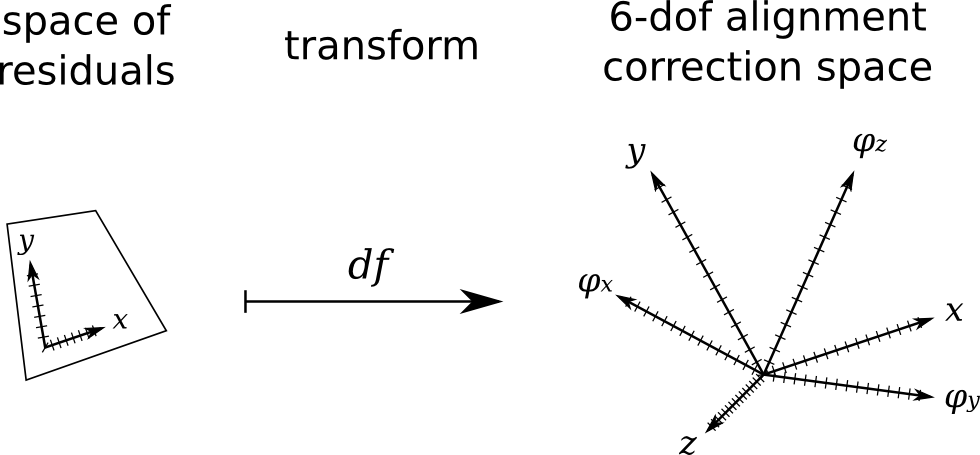
\includegraphics[width=\linewidth]{transformation.png}

\column{0.35\linewidth}
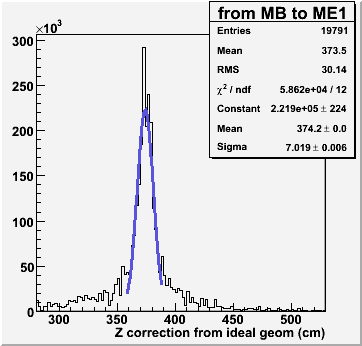
\includegraphics[width=\linewidth]{hist_0and1.png}
\end{columns}

\begin{itemize}
\item Normal HIP: weighted mean of residuals in correction space
\item Ntuple: ``every hit tells us where it thinks the disk is''
\item Without $\vec{B}$, we can't eliminate bad low-$\vec{p}$ tracks
\item Use weighted {\it mode} instead (best tracks agree and pile up)
\end{itemize}
\end{frame}

\begin{frame}
\frametitle{Results for CRUZETs 1\&2}
\small

\begin{columns}
\column{0.64\linewidth}
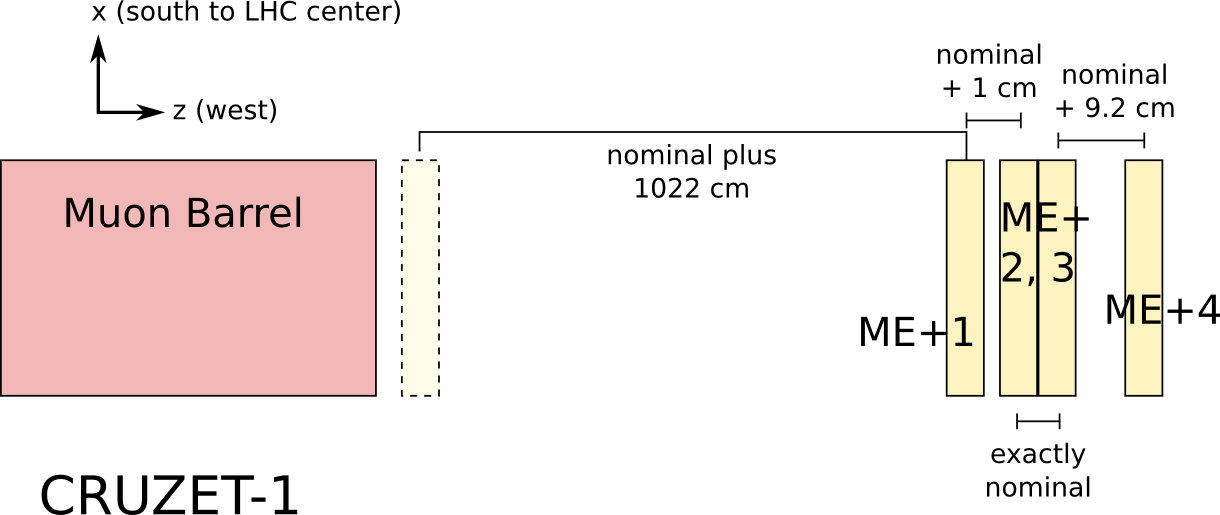
\includegraphics[height=3 cm]{cruzet1_results.png}

\vspace{0.5 cm}
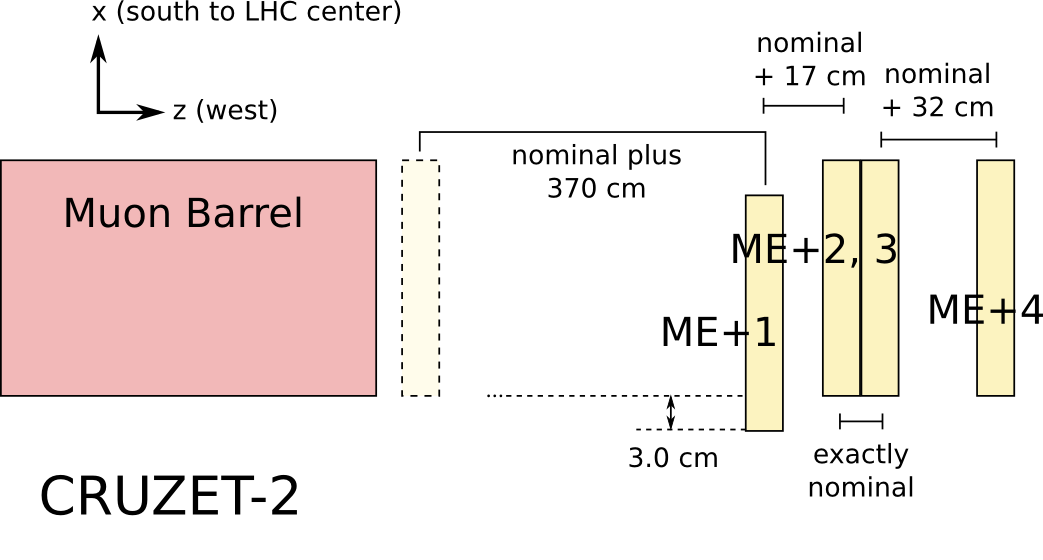
\includegraphics[height=3.3 cm]{cruzet2_results.png}

\column{0.4\linewidth}

\vspace{0.35 cm}
Observed all parameters, corrected and iterated \mbox{$xyz(\phi_z)$\hspace{-0.5 cm}}

\vspace{0.35 cm}
Few significant deviations from zero

\vspace{0.35 cm}
Significance defined by consistency of independent fits: 8~mm in $x$-$y$, 3~cm in $z$, few~mrad angles

\vspace{0.35 cm}
Tags for CSCAlignmentRcds:

\vspace{0.1 cm}
{\tt \tiny CRUZET1-CSCStation-xyz-2mmRadialFix\_v1

CRUZET2-CSCStation-xyzphiz-2mmRadialFix\_v2}

\vspace{0.35 cm}
Appropriate IOVs applied (thanks, Pablo!)
\end{columns}

\vspace{0.4 cm}
Details (soon): \textcolor{blue}{\tt \scriptsize \underline{\href{https://twiki.cern.ch/twiki/bin/view/CMS/MuonAlignment}{https://twiki.cern.ch/twiki/bin/view/CMS/MuonAlignment}}}
\end{frame}

\begin{frame}
\frametitle{Correction of ME2/2 and 3/2}
\small

Investigating the closure problems in CSC-Overlaps,

we found a mistake in the ideal CSCGeometry

\vfill
\begin{columns}
\column{0.4\linewidth}
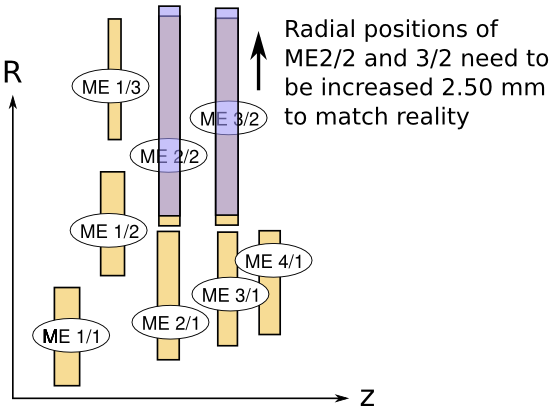
\includegraphics[width=\linewidth]{expand_ME22_32.png}

\column{0.6\linewidth}
\begin{itemize}
\item Discrepancy between drawings and DDD description of active volumes
\item Correction included in CRUZET alignments (``{\tt \scriptsize 2mmRadialFix}'')
\item DDD fix in the 2\_1\_1 release, which means that 2\_1\_X MC will be generated at the right positions
\end{itemize}
\end{columns}

\vspace{0.1 cm}
\begin{itemize}
\item Created new ideal CSCAlignmentRcd for reconstructing MC: {\tt \scriptsize CSCIdealGeometry211\_mc}

\vspace{0.1 cm}
Generated misalignment scenarios centered on corrected positions: {\tt \scriptsize CSC1InversepbScenario211v1\_mc}, {\tt \scriptsize CSC10InversepbScenario211v1\_mc}, etc.

\item Included in global tags {\tt \scriptsize IDEAL\_V6} and the {\tt \scriptsize STARTUP\_V5} for the 2\_1\_X

MC production
\end{itemize}
\end{frame}

\begin{frame}
\frametitle{New AlCaReco streams}
\small

To automate the procedure in CRUZET-4/CRAFT,

we need cosmic ray AlCaRecos:
\begin{itemize}\setlength{\itemsep}{0.3 cm}
\item ALCARECOMuAlStandAloneCosmics \hfill \begin{minipage}{3.5 cm}
$\displaystyle \left\}\begin{array}{l} \mbox{ } \\ \mbox{\scriptsize CommonAlignmentProducer} \\ \mbox{\scriptsize V00-30-06} \\ \mbox{ } \end{array}\right.$

\vspace{-1 cm} \mbox{ } \end{minipage}
\item ALCARECOMuAlGlobalCosmics
\item ALCARECOMuAlZeroFieldGlobalCosmics \hspace{0.27 cm} {\bf \}} {\scriptsize already published}
\end{itemize}

\vfill
Reasons:
\begin{itemize}
\item no minimum $p_T$ cut: essential for zero-field data
\item looser $\eta$ constraints ($\pm$100 instead of 2.4)
\item standard ALCARECOMuAlCalIsolatedMu is GlobalMuon-only: tracks that don't point into the tracker are also useful
\item special ZeroFieldGlobalCosmics because there are sometimes problems with tracker-to-muon matching in $\vec{B}=0$
\end{itemize}

\vfill
Limited testing (4000 CRUZET-3 events in 2\_0\_12)
\end{frame}


%% \section*{First section}
%% \begin{frame}
%% \begin{center}
%% \Huge \textcolor{blue}{First section}
%% \end{center}
%% \end{frame}

\begin{frame}
\frametitle{Summary/Conclusions}
\small

\begin{itemize}\setlength{\itemsep}{0.3 cm}
\item Still making progress on CSC-Overlaps procedure (it's subtle)
\item Corrected largest part of CSC misalignment: positions of
  disks relative to barrel (by a different method than Riccardo's)
  and positions of disks relative to one another (new, and large)
\item Will repeat barrel-to-endcap alignment in CRUZET-3 and add
  tracker-to-muon system (higher resolution and a different
  statistical distribution, perhaps alignment of some individual chambers)
\item Found an error in ideal geometry; added correction to CRUZET
  constants, fixed code for 2\_1\_1, updated MC ideal/misaligned
  geometries to match
\item New AlCaRecos needed for CRUZET-4/CRAFT
\end{itemize}

\label{numpages}
\end{frame}

\end{document}
